% Template of basic phisics experiment 基于 article template，在此基础上做修改
% 设定文章编码类型，正文字号为五号则 zihao=5，正文字号为小四则 zihao=-4
\documentclass[zihao=5, UTF8]{article}		


% 自定义宏定义
\def\N{\mathbb{N}}
\def\F{\mathbb{F}}
\def\Z{\mathbb{Z}}
\def\Q{\mathbb{Q}}
\def\R{\mathbb{R}}
\def\C{\mathbb{C}}
\def\T{\mathbb{T}}
\def\S{\mathbb{S}}
\def\A{\mathbb{A}}
\def\I{\mathscr{I}}
\def\d{\mathrm{d}}
\def\p{\partial}


% 物理实验报告所需的其它宏包
\usepackage{ulem}   % \uline 下划线支持

% 导入基本宏包
\usepackage[UTF8]{ctex}     % 设置文档为中文语言
\usepackage[colorlinks, linkcolor=blue, anchorcolor=blue, citecolor=blue, urlcolor=blue]{hyperref}  % 宏包：自动生成超链接 (此宏包与标题中的数学环境冲突)
% \usepackage{docmute}    % 宏包：子文件导入时自动去除导言区，用于主/子文件的写作方式，\include{./51单片机笔记}即可。注：启用此宏包会导致.tex文件capacity受限。
\usepackage{amsmath}    % 宏包：数学公式
\usepackage{mathrsfs}   % 宏包：提供更多数学符号
\usepackage{amssymb}    % 宏包：提供更多数学符号
\usepackage{pifont}     % 宏包：提供了特殊符号和字体
\usepackage{extarrows}  % 宏包：更多箭头符号

% 列表环境设置
\usepackage{enumitem}   % 宏包：列表环境设置
    \setlist[enumerate]{itemsep=0pt, parsep=0pt, topsep=0pt, partopsep=0pt, leftmargin=3.5em} 
    \setlist[itemize]{itemsep=0pt, parsep=0pt, topsep=0pt, partopsep=0pt, leftmargin=3.5em}
    \newlist{circledenum}{enumerate}{1} % 创建一个新的枚举环境  
    \setlist[circledenum,1]{  
        label=\protect\circled{\arabic*}, % 使用 \arabic* 来获取当前枚举计数器的值，并用 \circled 包装它  
        ref=\arabic*, % 如果需要引用列表项，这将决定引用格式（这里仍然使用数字）
        itemsep=0pt, parsep=0pt, topsep=0pt, partopsep=0pt, leftmargin=3.5em
    }  
% 文章页面 margin 设置
\usepackage[a4paper]{geometry}  % 宏包：文章页面 margin 设置
    \geometry{top=0.75in}
    \geometry{bottom=0.75in}
    \geometry{left=0.75in}
    \geometry{right=0.75in}   % 设置上下左右页边距
    \geometry{marginparwidth=1.75cm}    % 设置边注距离（注释、标记等）

% 自定义数学环境
\usepackage{amsthm} % 宏包：数学环境配置
% theorem-line 环境自定义
    \newtheoremstyle{MyLineTheoremStyle}% <name>
        {11pt}% <space above>
        {11pt}% <space below>
        {}% <body font> 使用默认正文字体
        {}% <indent amount>
        {\bfseries}% <theorem head font> 设置标题项为加粗
        {：}% <punctuation after theorem head>
        {.5em}% <space after theorem head>
        {\textbf{#1}\thmnumber{#2}\ \ (\,\textbf{#3}\,)}% 设置标题内容顺序
    \theoremstyle{MyLineTheoremStyle} % 应用自定义的定理样式
    \newtheorem{LineTheorem}{Theorem.\,}
% theorem-block 环境自定义
    \newtheoremstyle{MyBlockTheoremStyle}% <name>
        {11pt}% <space above>
        {11pt}% <space below>
        {}% <body font> 使用默认正文字体
        {}% <indent amount>
        {\bfseries}% <theorem head font> 设置标题项为加粗
        {：\\ \indent}% <punctuation after theorem head>
        {.5em}% <space after theorem head>
        {\textbf{#1}\thmnumber{#2}\ \ (\,\textbf{#3}\,)}% 设置标题内容顺序
    \theoremstyle{MyBlockTheoremStyle} % 应用自定义的定理样式
    \newtheorem{BlockTheorem}[LineTheorem]{Theorem.\,} % 使用 LineTheorem 的计数器
% definition 环境自定义
    \newtheoremstyle{MySubsubsectionStyle}% <name>
        {11pt}% <space above>
        {11pt}% <space below>
        {}% <body font> 使用默认正文字体
        {}% <indent amount>
        {\bfseries}% <theorem head font> 设置标题项为加粗
        {：\\ \indent}% <punctuation after theorem head>
        {0pt}% <space after theorem head>
        {\textbf{#3}}% 设置标题内容顺序
    \theoremstyle{MySubsubsectionStyle} % 应用自定义的定理样式
    \newtheorem{definition}{}


% 有色文本框及其设置
\usepackage[dvipsnames,svgnames]{xcolor}    %设置插入的文本框颜色
\usepackage[strict]{changepage}     % 提供一个 adjustwidth 环境
\usepackage{framed}     % 实现方框效果
    \definecolor{graybox_color}{rgb}{0.95,0.95,0.96} % 文本框颜色。修改此行中的 rgb 数值即可改变方框纹颜色，具体颜色的rgb数值可以在网站https://colordrop.io/ 中获得。（截止目前的尝试还没有成功过，感觉单位不一样）（找到喜欢的颜色，点击下方的小眼睛，找到rgb值，复制修改即可）
    \newenvironment{graybox}{%
    \def\FrameCommand{%
    \hspace{1pt}%
    {\color{gray}\small \vrule width 2pt}%
    {\color{graybox_color}\vrule width 4pt}%
    \colorbox{graybox_color}%
    }%
    \MakeFramed{\advance\hsize-\width\FrameRestore}%
    \noindent\hspace{-4.55pt}% disable indenting first paragraph
    \begin{adjustwidth}{}{7pt}%
    \vspace{2pt}\vspace{2pt}%
    }
    {%
    \vspace{2pt}\end{adjustwidth}\endMakeFramed%
    }

% 各级标题自定义设置
\usepackage{titlesec}   
    % section标题自定义设置 
    \titleformat{\section}[hang]{\normalfont\huge\bfseries\centering}{第\,\thesection\,部分}{20pt}{}
    % subsection标题自定义设置 
    \titleformat{\subsection}[hang]{\normalfont\Large\bfseries}{\,\thesubsection\,}{8pt}{}
    % subsubsection标题自定义设置
    \titleformat{\subsubsection}[hang]{\normalfont\large\bfseries}{\,\thesubsubsection\,}{6pt}{}

% 外源代码插入设置
\usepackage{matlab-prettifier}
    \lstset{
        style=Matlab-editor,  % 继承matlab代码颜色等
    }
\usepackage[most]{tcolorbox} % 引入tcolorbox包 
\usepackage{listings} % 引入listings包
    \tcbuselibrary{listings, skins, breakable}
    \lstdefinestyle{matlabstyle}{
        language=Matlab,
        basicstyle=\small,
        breakatwhitespace=false,
        breaklines=true,
        captionpos=b,
        keepspaces=true,
        numbers=left,
        numbersep=15pt,
        showspaces=false,
        showstringspaces=false,
        showtabs=false,
        tabsize=2
    }
    \newtcblisting{matlablisting}{
        arc=0pt,
        top=0pt,
        bottom=0pt,
        left=1mm,
        listing only,
        listing style=matlabstyle,
        breakable,
        colback=white   % 选一个合适的颜色
    }

% table 支持
\usepackage{booktabs}   % 宏包：三线表
\usepackage{tabularray} % 宏包：表格排版
\usepackage{longtable}  % 宏包：长表格
\usepackage{tabularx}  % 宏包：宽表格
\usepackage{multirow}  % 宏包：表格中一格显示多个项目

% figure 设置
\usepackage{graphicx}  % 支持 jpg, png, eps, pdf 图片 
\usepackage{svg}       % 支持 svg 图片
    \svgsetup{
        % 指向 inkscape.exe 的路径
        inkscapeexe = C:/aa_MySame/inkscape/bin/inkscape.exe, 
        % 一定程度上修复导入后图片文字溢出几何图形的问题
        inkscapelatex = false                 
    }


% 图表进阶设置
\usepackage{float}     % 图表位置浮动设置 
\usepackage{caption}    % 图注、表注
    \captionsetup[figure]{name=图}  
    \captionsetup[table]{name=表}
    \captionsetup{labelfont=bf, font=small}

% 文章默认字体设置
    \usepackage{fontspec}   % 宏包：字体设置
       \setmainfont{SimSun}    % 设置中文字体为宋体字体
      \setCJKmainfont[AutoFakeBold=3]{SimSun} % 设置加粗字体为 SimSun 族，AutoFakeBold 可以调整字体粗细^     \setmainfont{Times New Roman} % 设置英文字体为Times New Roman


% 其它设置
    % equation 公式编号设置
        \makeatletter  
        \renewcommand{\theequation}{\thesection.\arabic{equation}}  
        \makeatother
    % 脚注设置
        \renewcommand\thefootnote{\ding{\numexpr171+\value{footnote}}}
    % 参考文献引用设置
        \bibliographystyle{unsrt}   % 设置参考文献引用格式为unsrt
        \newcommand{\upcite}[1]{\textsuperscript{\cite{#1}}}     % 自定义上角标式引用
    % 文章序言设置
        \newcommand{\cnabstractname}{序言}
        \newenvironment{cnabstract}{%
            \par\Large
            \noindent\mbox{}\hfill{\bfseries \cnabstractname}\hfill\mbox{}\par
            \vskip 2.5ex
            }{\par\vskip 2.5ex}


% 页眉页脚设置
\usepackage{fancyhdr}   %宏包：页眉页脚设置
    \pagestyle{fancy}
    \fancyhf{}
    \cfoot{\thepage}
    \renewcommand\headrulewidth{1pt}
    \renewcommand\footrulewidth{0pt}
    \rhead{\bfseries 分组序号: YK04-2}    
    \chead{《基础物理实验》实验报告,\ 韩初晓,\ 2023K8009908002}
    \lhead{2024.10.10}

% 文档信息设置
%\title{这里是标题\\The Title of the Report}
%\author{丁毅\\ \footnotesize 中国科学院大学，北京 100049\\ Yi Ding \\ %\footnotesize University of Chinese Academy of Sciences, Beijing %100049, China}
%\date{\footnotesize 2024.8 -- 2025.1}

% 开始编辑文章

\begin{document}
\noindent\begin{flushright}
    \zihao{2}{分组序号: YK04-2}
\end{flushright}

\setCJKfamilyfont{boldsong}[AutoFakeBold = {2.17}]{SimSun}
\newcommand*{\boldsong}{\CJKfamily{boldsong}}


\begin{center}\large
    \noindent{\Huge\bfseries\boldsong《基础物理实验》实验报告 }
    \\\vspace{0.4cm}
    \noindent\textit{
        \textbf{\boldsong 实验名称：}\uline{\hspace{1.7cm} 温度与热导率测量\hspace{1.7cm}}\hspace{0.4cm} 
        指导教师：\uline{\hspace{1.0cm}李赫\hspace{1.0cm}}}
    \\\vspace{0.1cm}
    \noindent\textit{
        姓名：\uline{\,\,\,韩初晓\,\,\,}\hspace{0.2cm}
        学号：\uline{\,\,\,{\upshape 2023K8009908002}\,\,\,}\hspace{0.2cm}
        专业：\uline{\,\,\,计算机科学与技术\,\,\,}\hspace{0.2cm}
        班级：\uline{\,\,\,\upshape{2306}\,\,\,}}
    \\\vspace{0.1cm}
    \noindent\textit{
        实验日期：\uline{\,\,{\upshape 2024.10.10}\,\,}\hspace{0.2cm}
        实验地点：\uline{\,\,\,教学楼{\upshape427}\,\,\,}\hspace{0.2cm}
        是否调课/补课：\uline{\hspace{0.5cm}否\hspace{0.5cm}}\hspace{0.2cm}
        成绩：\uline{\hspace{2cm}}}
\end{center}
% \vspace{-0.2cm}
\noindent\rule{\textwidth}{0.1em}   % 分割线

% 控制目录不换页
\vspace{1cm}
\setcounter{tocdepth}{2}  % 目录深度为 2（不显示 subsubsection）
\noindent\begin{minipage}{\textwidth}\centering
\tableofcontents\thispagestyle{fancy}   % 显示页码、页眉等   
\end{minipage}  
\newpage

\section{实验目的}\thispagestyle{fancy} 

\subsection{动态法测定良导体的热导率}

\begin{enumerate}
  \item 通过实验学会一种测量热导率的方法。
  \item 解动态法的特点和优越性。
  \item 认识热波，加强对波动理论的理解。
\end{enumerate}

\subsection{温度的测量和温度计的设计}

\begin{enumerate}
  \item 用电位差计测热电偶的温差电动势。
  \item 用平衡电桥测热敏电阻和铜电阻的温度特性曲线。
  \item 设计非平衡电桥实现对热敏电阻的实时测量。
\end{enumerate}

\section{动态法测定良导体的热导率}

\subsection{实验用具}

\begin{table}[H]
\centering
\begin{tabular}{|c|l|}
\hline
\textbf{仪器组成部分} & \textbf{功能说明} \\ \hline
样品单元 & 用绝热材料紧裹侧表面的圆棒状样品（铜和铝两种样品）。 \\ \hline
热电偶列阵（传感器） & 测量棒体内轴线处的温度分布。 \\ \hline
脉动热源及冷却装置 & 实现边界条件，冷却水用于保持棒尾的温度$T_0$恒定。 \\ \hline
控制单元 & 控制仪器操作，调整实验参数。 \\ \hline
记录单元 & 
\begin{tabular}[c]{@{}l@{}} 
手动方式：使用高精度x-y记录仪；\\ 
程控方式：使用微机进行系统控制、数据采集、记录与绘图，\\ 学生自行处理数据。 
\end{tabular} \\ \hline
\end{tabular}
\caption{实验仪器组成及功能}
\end{table}

\begin{figure}[H]
    \centering
    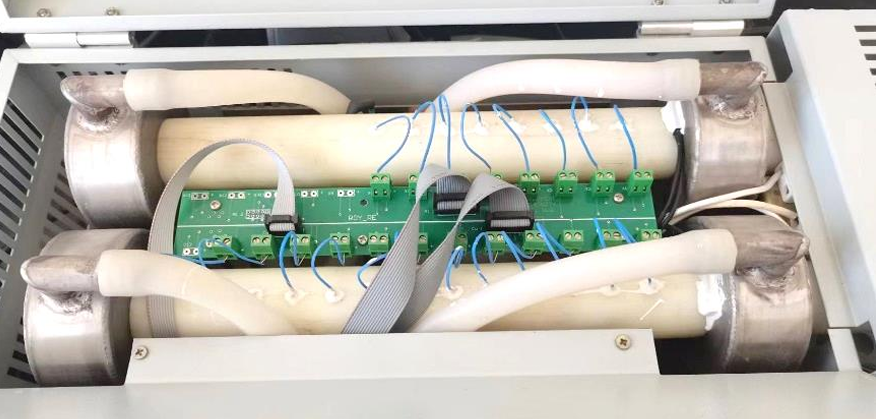
\includegraphics[width=0.6\textwidth]{./主机结构示意图.png}
    \caption{主机结构示意图}
\end{figure}

\begin{figure}[H]
    \centering
    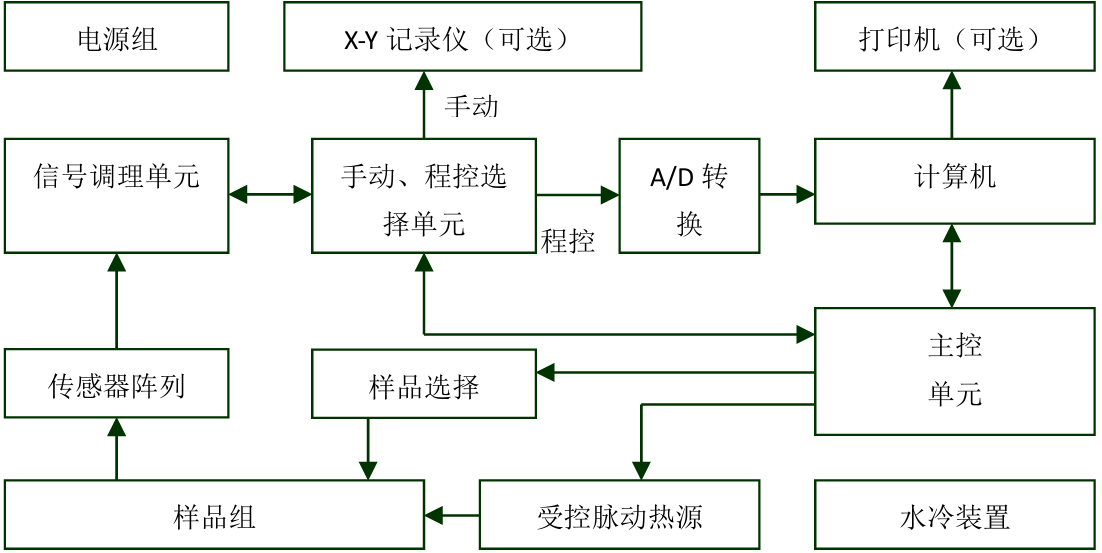
\includegraphics[width=0.6\textwidth]{./热导率动态测量过程示意图.png}
    \caption{热导率动态测量过程示意图}
\end{figure}


\subsection{实验原理}

为了简化问题，假设热量沿一维方向传播，样品制成棒状且周围隔热。考虑样品的一小段，如图3所示。根据热传导定律，单位时间内通过垂直于传播方向的面积$A$的热量，即热流为：

\begin{equation}
\frac{dq}{dt} = -kA \frac{dT}{dx}
\end{equation}

其中，$k$为材料的热导率，$A$为截面积，$\frac{dT}{dx}$为温度梯度。对上式两边同时取微分，得到：

\begin{equation}
\frac{d}{dt} \left(\frac{dq}{dt}\right) = -kA \frac{d^2 T}{dx^2} dx
\end{equation}

根据能量守恒，棒元的热平衡方程为：

\begin{equation}
C \rho A dx \frac{dT}{dt} = -kA \frac{d^2 T}{dx^2} dx
\end{equation}

其中，$C$和$\rho$分别为材料的比热容和密度。由此得到热流方程：

\begin{equation}
\frac{dT}{dt} = D \frac{d^2 T}{dx^2}
\end{equation}

其中，$D = \frac{k}{C \rho}$是热扩散系数。

上式的解表示了不同点温度随时间的变化，解的形式由边界条件决定。假设热端温度按简谐变化：

\begin{equation}
T = T_0 + T_m \sin (\omega t)
\end{equation}

另一端保持恒定低温$T_0$，则棒中各点的温度为：

\begin{equation}
T = T_0 - \alpha x + T_m e^{-\sqrt{\frac{\omega}{2D}} x} \sin \left(\omega t - \sqrt{\frac{\omega}{2D}} x \right)
\end{equation}

其中，$T_0$是直流成分，$\alpha$为温度梯度。从上式可以得出以下结论：

\begin{itemize}
    \item 热端（$x=0$）处的温度按简谐变化，热波沿棒传播并逐渐衰减。
    \item 热波的波速为：$V = \sqrt{2D \omega}$。
    \item 热波的波长为：$\lambda = 2\pi \sqrt{\frac{2D}{\omega}}$。
\end{itemize}

在已知热端温度变化的频率$\omega$时，测量波速$V$或波长$\lambda$即可计算热扩散系数$D$，进而计算材料的热导率$k$。由此得到：

\begin{equation}
V^2 = 2 \frac{k}{C \rho} \omega \quad \Rightarrow \quad k = \frac{V^2 C \rho}{4 \pi f}
\end{equation}

其中，$f$为热端温度变化的频率，$T$为周期。测量的关键在于：a) 热量在样品中一维传播；b) 热端温度按简谐变化。

\subsection{实验内容}

\subsubsection*{1. 检查与准备工作}
\begin{enumerate}
    \item 检查各连接管路，确保无堵塞，然后开启水源。
    \item 打开仪器盖子，阅读注意事项。
\end{enumerate}

\subsubsection*{2. 水流调节}
\begin{enumerate}
    \item 打开水源，观察水流稳定，阀门开至1/3开度。
    \item 热端水流量适中，保持温度稳定，避免波动。
    \item 冷端水流量不要求太高，保持室温即可。
    \item 观察软件数据显示曲线的幅度和形状，调节水流。
    \item 冷却水管串联，先测铜棒后测铝棒，避免水变热。
\end{enumerate}

\subsubsection*{3. 电源开启与工作设置}
\begin{enumerate}
    \item 打开电源开关，进入工作状态。
    \item 选择“程控”工作方式，调节好水流。
    \item 进入软件，设置热源周期 $T$（一般为180秒）。
    \item 选择铜棒或铝棒进行测量，建议先测铜后测铝。
    \item 设置软件中的x、y轴单位：x轴为时间（秒），y轴为信号强度（毫伏）。
    \item 选择测量点，按下“测量”按钮开始实验。
\end{enumerate}

\subsubsection*{4. 数据记录与结束操作}
\begin{enumerate}
    \item 实验进行40分钟，系统进入动态平衡，样品温度稳定。
    \item 按“暂停”按钮，保存数据或打印曲线。
    \item 不要使用“平滑”功能，避免信号失真。
    \item 实验结束后，依次关闭测量仪器、水源和电脑，避免仪器因缺水冷却而损坏。
\end{enumerate}

\subsection{数据整理与计算}

\subsubsection{热波波速的测量}

\begin{table}[H]
    \centering
    \begin{tabular}{|c|c|c|c|c|c|c|}
    \hline
        测量点n & 1 & 2 & 3 & 4 & 5 & 6 \\ \hline
        对应峰值时间t (s) & 1538.04 & 1542.52 & 1548.52 & 1556.04 & 1566.04 & 1572.04 \\ \hline
        波速$(\times10^{-3}m/s)$ & 4.464 & 3.333 & 2.660 & 2.000 & 3.333 & ~ \\ \hline
        \multicolumn{3}{|c|}{波速平均值：3.158$\times10^{-3}m/s$} & ~ & \multicolumn{3}{c|}{热导率：$490.832 \mathrm{W/(m \cdot K)}$} \\ \hline
    \end{tabular}
    \caption{动态法测铜的热导率}
\end{table}

代入数据 $C_\text{铜}=0.385\ \mathrm{J/(g \cdot K)}$, $\rho_\text{铜}=8.92\times10^6\ \mathrm{g/m^3}$, $T=180\ \mathrm{s}$ 得：
\[
k = \frac{V^2 C \rho}{4\pi f} = \frac{V^2 C \rho}{4\pi} T = 490.832\ \mathrm{W/(m \cdot K)}
\]

查到铜的热导率为 $401\ \mathrm{W/(m \cdot K)}$, 相对误差 $22.40\%$。


\begin{table}[H]
    \centering
    \begin{tabular}{|c|c|c|c|c|c|c|}
    \hline
        测量点n & 1 & 2 & 3 & 4 & 5 & 6 \\ \hline
        对应峰值时间t (s) & 4777.52 & 4783.04 & 4790.52 & 4799.52 & 4810.52 & 4820.04 \\ \hline
        波速$(\times10^{-3}m/s)$ & 3.623 & 2.674 & 2.222 & 1.818 & 2.101 & ~ \\ \hline
        \multicolumn{3}{|c|}{波速平均值：2.488$\times10^{-3}m/s$} & ~ & \multicolumn{3}{c|}{热导率：$215.461\ \mathrm{W/(m \cdot K)}$} \\ \hline
    \end{tabular}
    \caption{动态法测铝的热导率}
\end{table}

代入数据 $C_\text{铝}=0.9\ \mathrm{J/(g \cdot K)}$, $\rho_\text{铝}=2.7\times10^6\ \mathrm{g/m^3}$, $T=180\ \mathrm{s}$ 得：
\[
k = \frac{V^2 C \rho}{4\pi f} = \frac{V^2 C \rho}{4\pi} T = 215.461\ \mathrm{W/(m \cdot K)}
\]

查到铝的热导率为 $237\ \mathrm{W/(m \cdot K)}$, 相对误差 $9.09\%$。


\subsection{总结与思考}

\subsubsection*{1. 如果想知道某一时刻 $ t $ 时材料棒上的热波，即 $ T(x) $ 曲线，将如何做？}

为了确定某一时刻 $ t $ 时材料棒上的温度分布 $ T(x) $，可以按照以下步骤进行：

1. \textbf{选择时间点}：从保存的数据中选择一个特定的时间点 $ t $。
2. \textbf{读取电压值}：读出该时间点 $ t $ 对应的所有热电偶的电压值。
3. \textbf{电压-温度转换}：根据热电偶的电压-温度转换关系，将电压值转换为温度值。
4. \textbf{绘制温度分布曲线}：将每个位置的温度值 $ T(x) $ 绘制成曲线，从而得到该时刻的温度分布 $ T(x) $。

\subsubsection*{2. 为什么较后面测量点的 $ T(t) $ 曲线振幅越来越小？}

根据之前推算出的公式：

$$
T = T_0 - \alpha + T_m e^{-\sqrt{\frac{\omega x}{2D}}} \sin(\omega t - \frac{\omega}{2D} x)
$$

波的振幅为 $ T_m e^{-\sqrt{\frac{\omega x}{2D}}} $，其随距离 $ x $ 增大而不断衰减。具体来说：

1. \textbf{衰减因子}：随着距离 $ x $ 的增加，衰减因子 $ e^{-\sqrt{\frac{\omega x}{2D}}} $ 逐渐减小，导致振幅减小。
2. \textbf{直观理解}：热端的振幅来源于输入的简谐变化，冷端则是一恒定值。因此，越靠近热端，振幅越接近输入振幅；越靠近冷端，振幅越接近零。

\subsubsection*{3. 为什么实验中铝棒的测温点才8个，而铜棒的测温点达到12个？}

从实验所得的图像上来看：

1. \textbf{铝棒}：稳定后，铝在第8个采样点所测出的波振幅已经很不明显。根据之前算出的数据，铝的热扩散系数较小，衰减因子 $ e^{-\sqrt{\frac{\omega x}{2D}}} $ 在相同 $ x $ 情况下比铜大，铝8个采样点后振幅约为初始值的5\%左右，继续的测量已经没有意义。
2. \textbf{铜棒}：铜棒在第12个采样点所测出的波振幅仍然可以辨认出较明显的波峰和波谷。铜的热扩散系数较大，衰减因子较小，因此在12个采样点后振幅约为初始值的4\%，与铝8个采样点时的衰减程度接近。若采样点过少，则衰减不完全，虽不影响周期的测量，但会导致 $ T-x $ 图像不容易准确画出。

\subsubsection*{4. 实验中误差的来源有哪些？}

实验中误差的来源主要包括以下几个方面：

1. \textbf{根据数据判断波峰的位置时的读数误差}：在确定波峰位置时，读数可能存在误差。事实上，在对照实验数据时，经常出现在温度的最大值附近十几个测量点的电压值都相同的情况。
2. \textbf{热电偶本身的质量问题}：热电偶的质量问题可能导致测量不准确。
3. \textbf{热电偶测量的不准确}：热电偶本身的测量误差，包括温度-电压转换的误差。

\subsubsection*{5. 实验心得}

在上文计算过程中，铜的热导率为$490.832 \mathrm{W/(m \cdot K)}$,与理论值401\,$\mathrm{W/(m \cdot K)}$相比有较大误差，为此，使用逐差法重新计算铜的热波波速和热导率。具体步骤如下：

\textbf{实验数据} \\

\begin{table}[H]
    \centering
    \begin{tabular}{|c|c|c|c|c|c|c|}
    \hline
        测量点n & 1 & 2 & 3 & 4 & 5 & 6 \\ \hline
        对应峰值时间t (s) & 1538.04 & 1542.52 & 1548.52 & 1556.04 & 1566.04 & 1572.04 \\ \hline
    \end{tabular}
    \caption{动态法测铜的热导率}
\end{table}

已知参数：
\begin{itemize}
    \item 比热容 \( C_{\text{铜}} = 0.385\ \mathrm{J/(g \cdot K)} = 385\ \mathrm{J/(kg \cdot K)} \)
    \item 密度 \( \rho_{\text{铜}} = 8.92 \times 10^3\ \mathrm{kg/m^3} \)
    \item 周期 \( T = 180\ \mathrm{s} \)
    \item 位移 \( x = 18\ \mathrm{cm} = 0.18\ \mathrm{m} \)
\end{itemize}

\textbf{步骤一：计算时间差 \( \delta t \)} \\

\[
\delta t = (t_4 + t_5 + t_6) - (t_1 + t_2 + t_3)
\]

代入数据：

\[
\delta t = (1556.04\,\text{s} + 1566.04\,\text{s} + 1572.04\,\text{s}) - (1538.04\,\text{s} + 1542.52\,\text{s} + 1548.52\,\text{s}) = 4694.12\,\text{s} - 4629.08\,\text{s} = 65.04\,\text{s}
\]

\textbf{步骤二：计算波速 \( V \)} \\

波速的计算公式为：

\[
V = \frac{x}{\delta t}
\]

代入数据：

\[
V = \frac{0.18\,\mathrm{m}}{65.04\,\mathrm{s}} \approx 0.002773\,\mathrm{m/s}
\]

\textbf{步骤三：计算角频率 \( \omega \)} \\

角频率的计算公式为：

\[
\omega = \frac{2\pi}{T} = \frac{2\pi}{180} \approx 0.03491\,\mathrm{rad/s}
\]

\textbf{步骤四：计算热扩散系数 \( D \)} \\

热扩散系数与波速的关系为：

\[
V = \sqrt{2D\omega} \quad \Rightarrow \quad D = \frac{V^2}{2\omega}
\]

代入计算：

\[
D = \frac{(0.002773\,\mathrm{m/s})^2}{2 \times 0.03491\,\mathrm{rad/s}} = \frac{7.691 \times 10^{-6}\,\mathrm{m^2/s^2}}{0.06982\,\mathrm{rad/s}} \approx 1.101 \times 10^{-4}\,\mathrm{m^2/s}
\]

\textbf{步骤五：计算热导率 \( k \)} \\

热导率的计算公式为：

\[
k = D \times C \times \rho
\]

代入已知数值：

\[
k = 1.101 \times 10^{-4}\,\mathrm{m^2/s} \times 385\,\mathrm{J/(kg \cdot K)} \times 8.92 \times 10^3\,\mathrm{kg/m^3}
\]

计算步骤：

\[
k = 1.101 \times 10^{-4} \times 385 \times 8.92 \times 10^3 \approx 378\,\mathrm{W/(m \cdot K)}
\]

\textbf{计算结果} \\

通过重新计算，得到铜的热导率为：

\[
k \approx 378\,\mathrm{W/(m \cdot K)}
\]

与已知铜的标准热导率 \( 401\,\mathrm{W/(m \cdot K)} \) 相比，存在约 5\% 的相对误差。这一结果与之前计算的结果相比，误差较小，说明逐差法计算的结果更加准确。




\section{温度的测量和温度计的设计}

\subsection{实验用具}

\subsubsection{DHT-2 热学实验装置温控仪}

\begin{figure}[H]
    \centering
    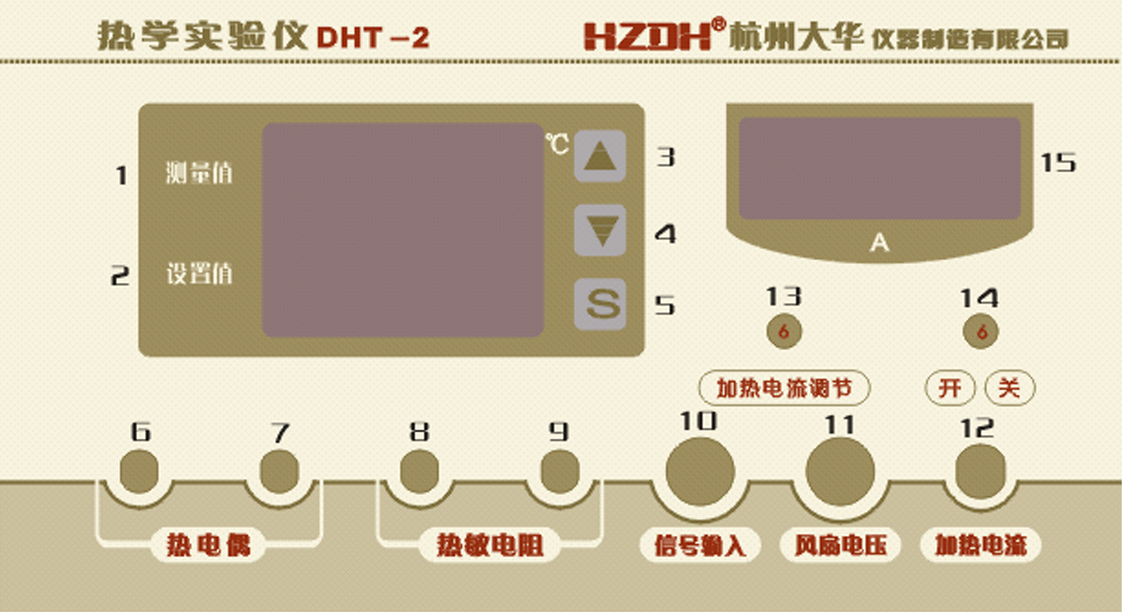
\includegraphics[width=0.6\textwidth]{./DHT-2 热学实验装置温控仪.png}
    \caption{DHT-2 热学实验装置温控仪}
\end{figure}

\begin{table}[H]
\centering
\begin{tabular}{|c|p{10cm}|}
\hline
1 & 测量值：显示器(绿) \\ \hline
2 & 设定值：显示器(红) \\ \hline
3 & 加数键(▲)：在温度设定时，作加数键。 \\ \hline
4 & 减数键(▼)：在温度设定时，作减数键。 \\ \hline
5 & 设定键(S)：设定值。按设定键(S)，SV显示器一位数码管闪烁，则该位进入修改状态，再按S键，闪烁位向左移一位，不按设定键(S)8秒(即数码管闪烁8秒)自动停止闪烁并返回至正常显示设定值。 \\ \hline
5-3 & 设定键(S)+加数键(▲)：组合键设定PID参数。 \\ \hline
5-4 & 设定键(S)+减数键(▼)：组合键设定PID参数。 \\ \hline
6-7 & 热电偶输出端子。 \\ \hline
8-9 & 热敏电阻输出端子(NTC) \\ \hline
10 & 加热电流输出插座。 \\ \hline
11 & 风扇电压输出插座。 \\ \hline
12 & 加热炉信号输入插座。 \\ \hline
13 & 加热电流调节电位器。 \\ \hline
14 & 加热电流输出控制开关。 \\ \hline
15 & 加热电流显示表。 \\ \hline
\end{tabular}
\caption{DHT-2 热学实验装置温控仪各接口定义}
\end{table}

\subsubsection{UJ36a型携带式直流电位差计}

\begin{figure}[H]
    \centering
    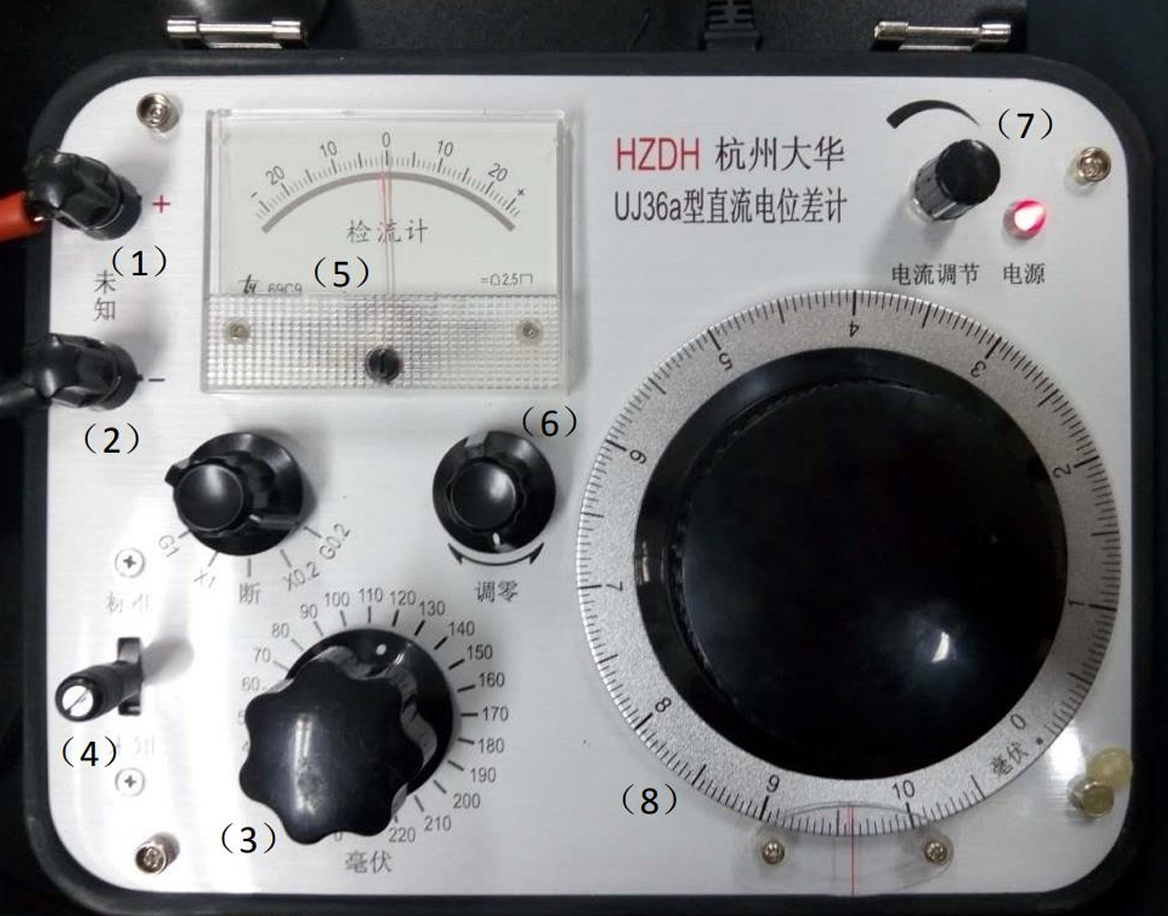
\includegraphics[width=0.6\textwidth]{./UJ36a型携带式直流电位差计.png}
    \caption{UJ36a型携带式直流电位差计}
\end{figure}

\begin{table}[ht]
\centering
\begin{tabular}{|c|l|}
\hline
(1)& 未知电压测量接线柱 \\ \hline
(2)& 倍率开关 \\ \hline
(3)& 步进盘(规盘) \\ \hline
(4)& 电键开关 \\ \hline
(5)& 检流计 \\ \hline
(6)& 检流计调零 \\ \hline
(7)& 工作电流调节变阻器 \\ \hline
(8)& 滑线盘 \\ \hline
\end{tabular}
\caption{UJ36a型携带式直流电位差计操作面板定义}
\end{table}

\subsubsection{DHQJ-5型教学用多功能电桥}

\begin{figure}[H]
    \centering
    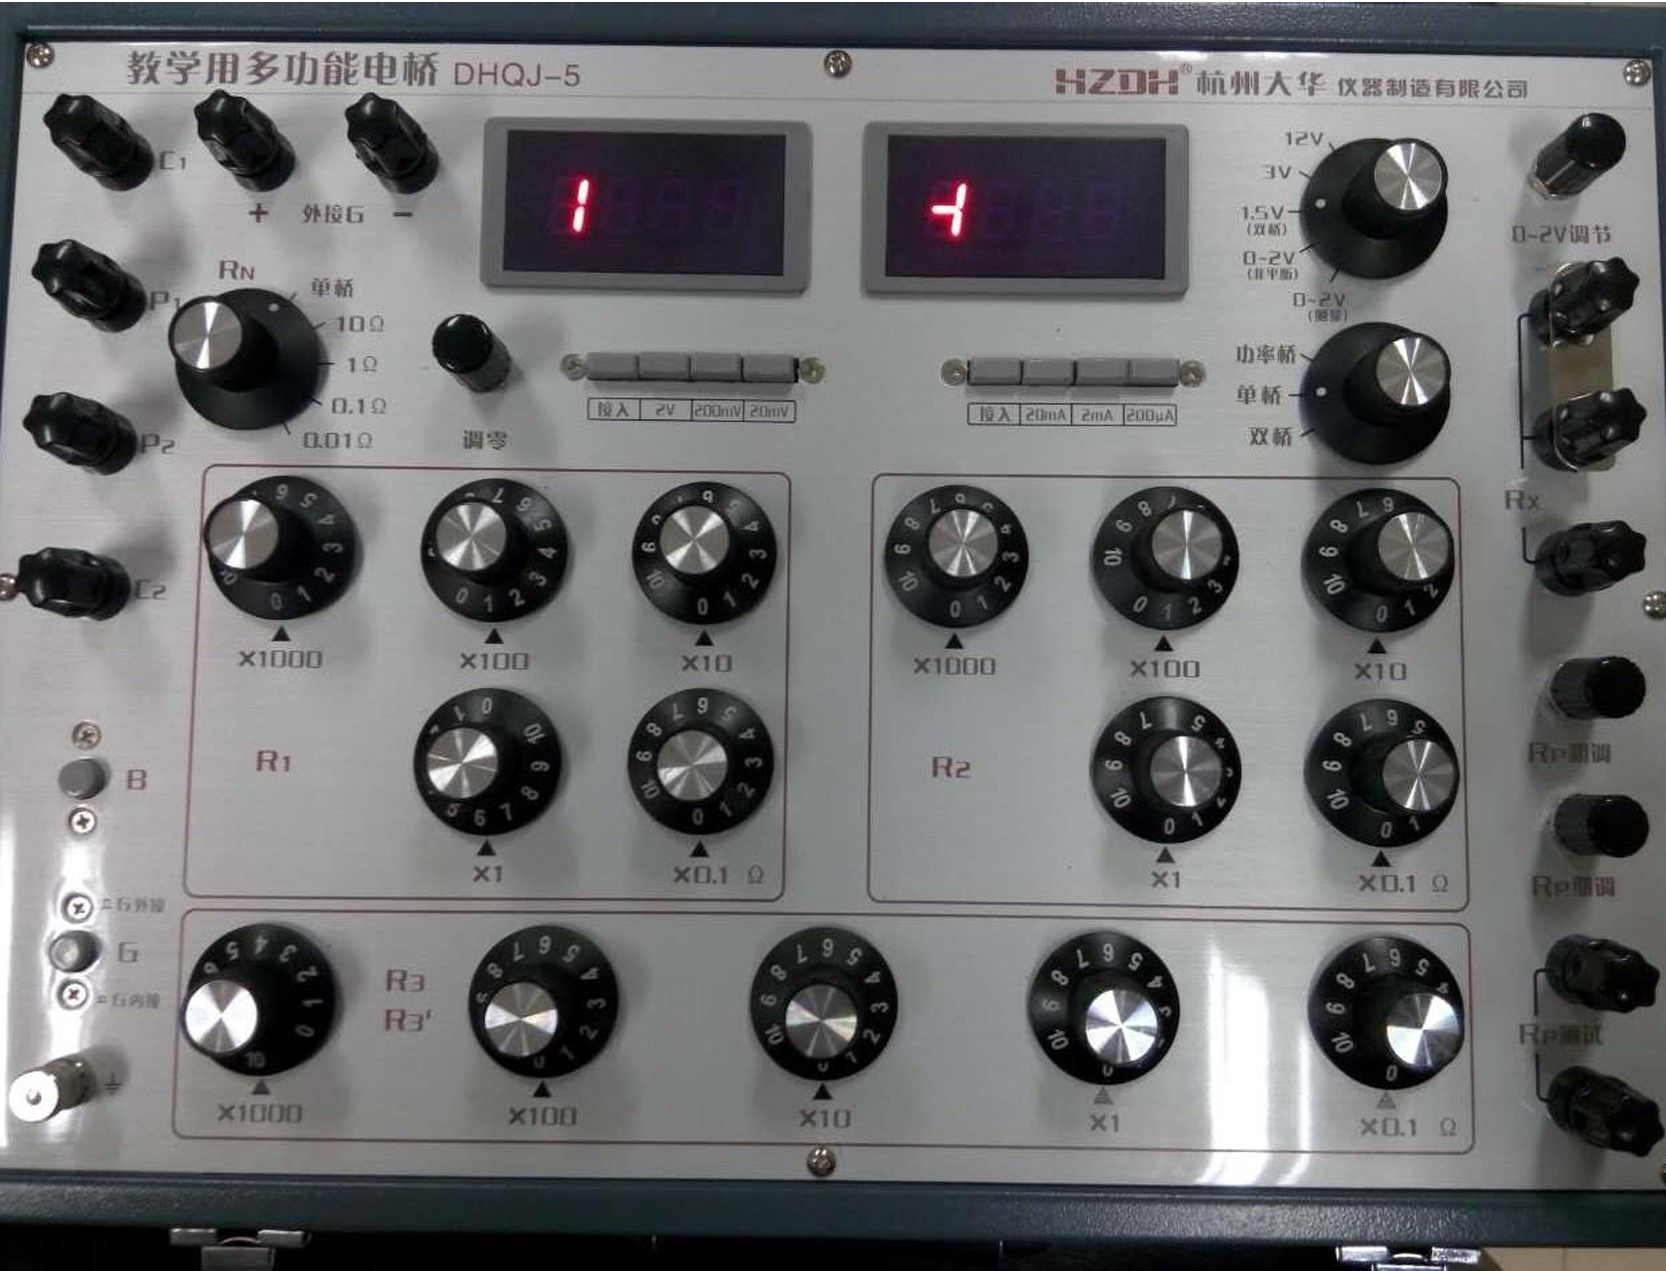
\includegraphics[width=0.6\textwidth]{./DHQJ-5型教学用多功能电桥.png}
    \caption{DHQJ-5型教学用多功能电桥}
\end{figure}

\begin{table}[h]
\centering
\label{tab:DHQJ-5型教学用多功能电桥}
\begin{tabular}{|c|c|c|c|c|}
\hline
\textbf{量程倍率} & \textbf{有效量程(Ω)} & \textbf{R1 (Ω)} & \textbf{R2 (Ω)} & \textbf{工作电压} \\ \hline
$\times10^{-3}$ & $1\sim11.111$ & 10000 & 10 & 3V \\ \hline
$\times10^{-2}$ & $10\sim111.11$ & 10000 & 100 & 3V \\ \hline
$\times10^{-1}$ & $100\sim1111.1$ & 10000 & 1000 & 3V \\ \hline
$\times1$ & $1K\sim11.111K$ & 1000 & 1000 & 3V \\ \hline
$\times10$ & $10K\sim111.11K$ & 1000 & 10000 & 3V \\ \hline
$\times10^{2}$ & $100K\sim1111.1K$ & 100 & 10000 & 12V \\ \hline
$\times10^{3}$ & $1M\sim11.111M$ & 10 & 10000 & 12V \\ \hline
\end{tabular}
\caption{单臂电桥技术参数和设定参考值}
\end{table}

\textbf{DHQJ-5型教学用多功能电桥的使用方法及注意事项：}


\begin{enumerate}
  \item \textbf{标准电阻$R_{\text{N}}$选择开关选择“单桥”档。}
  \item \textbf{工作方式开关选择“单桥”档。}
  \item \textbf{电源选择开关：} 建议按表2有效量程选择工作电源电压。
  \item \textbf{G开关选择“G内接”。}
  \item \textbf{根据$R_{X}$值估计值：} 按表2选择量程倍率，设置好$R_{1}$、$R_{2}$值和$R_{3}$值，将未知电阻$R_{X}$接入$R_{X}$接线端子。\\
  （注意：$R_{X}$端子上方短接片应接好。）
  \item \textbf{打开仪器市电开关，面板指示灯亮。}
  \item \textbf{建议选择毫伏表作为仪器检流计：} 释放“接入”按键，量程置“20mV”档，调节“调零”电位器，将数显表调零。调零后将量程转入200mV量程，按下“接入”按键，也可以选择微安表作检流计。
  \item \textbf{调节$R_{3}$各盘电阻：} 粗平衡后，可以选择200mV或20mV档，细调$R_{3}$位，使电桥平衡。
\end{enumerate}

\subsection{实验原理}

\subsubsection{用电位差计测热电偶的温差电动势}

热电偶是由 A、B 两种不同材料的金属丝的端点紧密接触组成的。当两个接点处于不同温度时（如图 \ref{fig:温差电偶示意图} 左图），在回路中会产生直流电动势，称为温差电动势或热电动势。测试电路如图 \ref{fig:热电偶温度计示意图} 所示。当组成热电偶的材料一定时，温差电动势 $ E_x $ 仅与两接点处的温度有关，并且两接点的温差在一定的温度范围内有如下近似关系式：

\begin{equation}
E_x \approx \alpha (t - t_0)
\end{equation}

式中 $\alpha$ 称为温差电系数，对于不同金属组成的热电偶，$\alpha$ 是不同的，其数值上等于两接点温度差为 1°C 时所产生的电动势。

为了测量温差电动势，需要在图 \ref{fig:热电偶温度计示意图}  的回路中接入电位差计，但测量仪器的引入不能影响热电偶原来的性质。根据伏打定律，即在 A、B 两种金属之间插入第三种金属 C 时，若它与 A、B 的两连接点处于同一温度 $t_0$（图 \ref{fig:温差电偶示意图} 右图），则该闭合回路的温差电动势与上述只有 A、B 两种金属组成回路时的数值完全相同。因此，我们把 A、B 两根不同化学成份的金属丝的一端焊在一起，构成热电偶的热端（工作端）。将另一端各与铜引线（即第三种金属 C）焊接，构成两个同温度 $t_0$ 的冷端（自由端）。

铜引线与电位差计相连，这样就组成一个热电偶温度计。通常将冷端置于冰水混合物中，保持 $t_0 = 0$ °C，将热端置于待测温度处，即可测得相应的温差电动势，再根据事先校正好的曲线或数据来求出温度 $t$。

\begin{figure}[H]
  \centering
  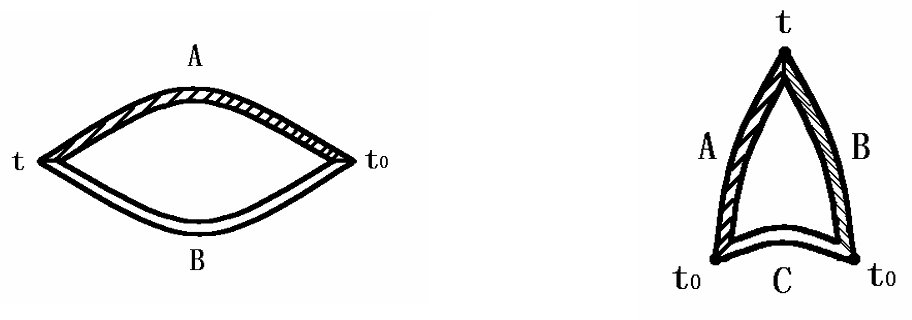
\includegraphics[width=0.6\textwidth]{./温差电偶示意图.png}
  \caption{温差电偶示意图}
  \label{fig:温差电偶示意图}
\end{figure}

\begin{figure}[H]
\centering
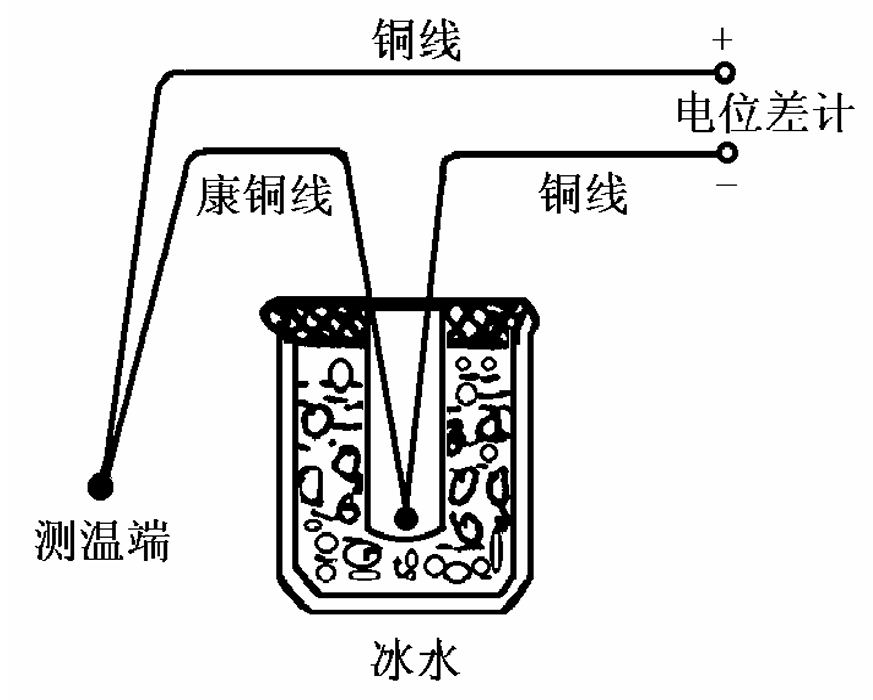
\includegraphics[width=0.3\textwidth]{./热电偶温度计示意图.png}
\caption{热电偶温度计示意图}
\label{fig:热电偶温度计示意图}
\end{figure}

\subsubsection{金属电阻温度计}

金属的电阻随温度的变化满足下式：

\begin{equation}
R_x = R_{x0} (1 + \alpha t + \beta t^2)
\label{eq:resistance_temp}
\end{equation}

对于铜电阻传感器，在$ t = 0 \, ^\circ \text{C} $时的电阻值为 $ R_{x0} = 50 \, \Omega $，其温度系数为：

\begin{equation}
\alpha = 4.289 \times 10^{-3} \, / \, ^\circ \text{C}, \quad \beta = -2.133 \times 10^{-7} \, / \, ^\circ \text{C}
\label{eq:coefficients}
\end{equation}

在温度不是很高情况下，忽略温度二次项 $\beta t^2$，可将金属的电阻值随温度变化视为线性变化，即：

\begin{equation}
R_x = R_{x0} (1 + \alpha t) = R_{x0} + \alpha t \, R_{x0}
\label{eq:linear_approximation}
\end{equation}

用控温仪将铜电阻的温度控制在一系列温度值上，待温度稳定后，用平衡电桥测出铜电阻的阻值，画出温度-阻值曲线，就可以得出铜电阻的温度特性曲线，进行线性拟合可以求出温度系数，这就是温度计的标定。

\subsubsection{半导体热敏温度计}

半导体热敏电阻（NTC）具有负的电阻温度系数，电阻随温度升高而下降。这是因为热敏电阻由金属氧化物（如 $\mathrm{Fe}_3\mathrm{O}_4$、$\mathrm{MgCr}_2\mathrm{O}_4$）制成，在温度升高时，自由电子数目增加，导电能力增强。

热敏电阻的电阻温度特性可以用以下指数函数描述：
\begin{equation}
R_T = A e^{\frac{B}{T}}
\end{equation}
其中，$A$ 为与材料和几何形状相关的常数，$B$ 为材料特性常数，$T$ 为绝对温度。

取对数得到：
\begin{equation}
\ln R_T = \ln A + \frac{B}{T}
\end{equation}

对于不同温度 $T_1$ 和 $T_2$，分别有：
\begin{equation}
\ln R_{T_1} = \ln A + \frac{B}{T_1}, \quad \ln R_{T_2} = \ln A + \frac{B}{T_2}
\end{equation}

相减得到 $B$ 的表达式：
\begin{equation}
B = \frac{\ln R_{T_1} - \ln R_{T_2}}{\frac{1}{T_1} - \frac{1}{T_2}}
\end{equation}

代入求得 $A$：
\begin{equation}
A = R_{T_1} e^{-\frac{B}{T_1}}
\end{equation}

常用的半导体热敏电阻的 $B$ 值约为 $1500 \sim 5000 \, \mathrm{K}$。

通过控制温度并使用平衡电桥测量不同温度下的电阻，可以利用上述公式拟合数据，求出热敏电阻的系数 $A$ 和 $B$。

金属电阻和热敏电阻的特性曲线示意图如图 \ref{fig:热敏电阻和金属电阻特性曲线} 所示。

\begin{figure}[H]
\centering
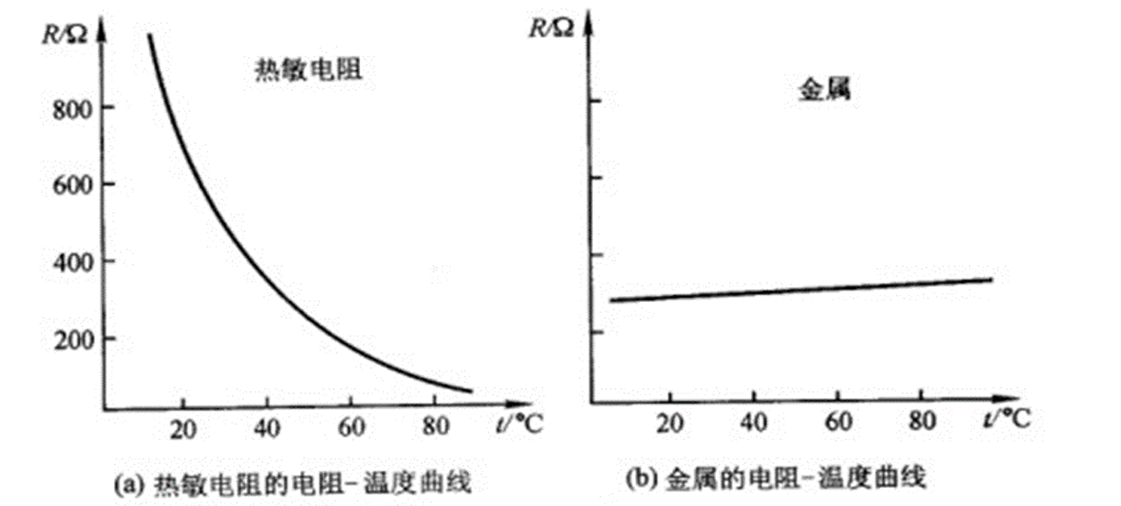
\includegraphics[width=0.6\textwidth]{./热敏电阻和金属电阻特性曲线.png}
\caption{热敏电阻和金属电阻特性曲线}
\label{fig:热敏电阻和金属电阻特性曲线}
\end{figure}

\subsubsection{设计非平衡电桥实现对热敏电阻的实时测量}

非平衡电桥的电路图与平衡电桥相似，见图  \ref{fig:non_balance_bridge} 。测试步骤与平衡电桥相同，只是使用电压表测量两端电压，忽略电压表内阻的影响。在平衡时电桥电压为 0，非平衡时电桥电压 $ U_0 $ 随 $ R_x $ 变化，通过选择合适的 $ R_1 $、$ R_2 $、$ R_3 $ 和 $ E $，使得测试电压 $ U_0 $ 随温度 $ T $ 线性变化，实现对温度的实时测量。

\begin{figure}[h]
    \centering
    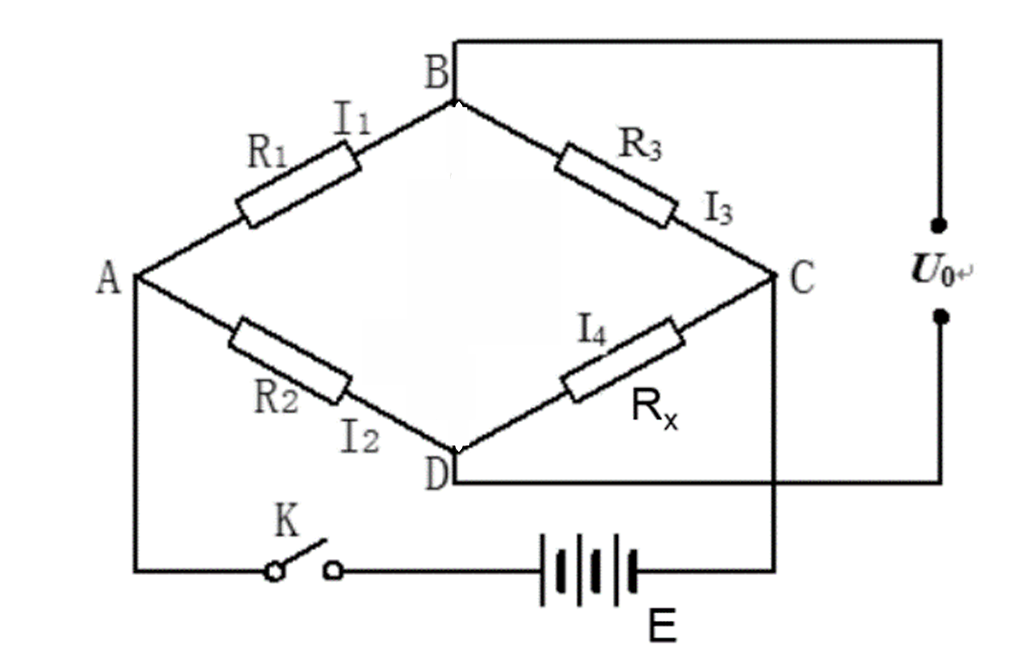
\includegraphics[width=0.6\textwidth]{./非平衡电桥电路图.png}
    \caption{非平衡电桥电路图}
    \label{fig:non_balance_bridge}
\end{figure}

电压表内阻假设为无穷大，电压 $ U_0 $ 为：

\begin{equation}
U_0 = \left( \frac{R_x}{R_x + R_s} - \frac{R_2}{R_1 + R_3} \right) E
\end{equation}

其中，$ R_x = A e^{\frac{B}{T}} $，$ A $ 和 $ B $ 通过平衡电桥在两个温度点测量得到。

将 $ R_x $ 代入电压公式得到 $ U_0 $ 与温度 $ T $ 的关系。对 $ U_0 $ 进行泰勒级数展开，保留到二阶项，忽略高阶项，得到：

\begin{equation}
U_0 = U_{01} + U_0' (T - T_i) + U_0'' (T - T_i)^2
\end{equation}

其中，$ T_i $ 为温度区间的中间值。令 $ U_0'' = 0 $，得到：

\begin{equation}
R_x = A e^{\frac{B}{T}} = \frac{B + 2T}{B - 2T} R_{2}
\end{equation}

然后，$ U_0 $ 可以表示为温度的线性函数：

\begin{equation}
U_0 = \lambda + m (T - T_i)
\end{equation}

\begin{equation}
\lambda = \left( \frac{B + 2T_i}{2B} - \frac{R_2}{R_1 + R_3} \right) E, \quad m = \left( \frac{4T_i^2 - B^2}{4BT_i^2} \right) E
\end{equation}

其中，$ \lambda $ 表示温度区间中间值时的电压，$ m $ 表示灵敏度。通过选择合适的 $ \lambda = -400 \, \text{mV} $ 和 $ m = 10 \, \text{mV/°C} $，可以通过测得的电压 $ U_0 $ 推算温度。

根据选择的 $ \lambda $ 和 $ m $，以及式（28），可以计算出 $ E $、$ R_2 $ 和 $ \frac{R_1}{R_3} $ 的值，具体如下：

\begin{equation}
E = \left( \frac{4BT_i^2}{4T_i^2 - B^2} \right) m
\end{equation}

\begin{equation}
R_x = \frac{B - 2T}{B + 2T} R_{x1}
\end{equation}

\begin{equation}
\frac{R_2}{R_3} = \frac{2BE}{(B + 2T_i)E - 2B\lambda} - 1
\end{equation}

通过计算得到的 $ E $、$ R_2 $ 和 $ R_1/R_3 $ 值，可以设置非平衡电桥的参数。调整控温仪至设定温度（例如 40°C），微调 $ R_x $，确保电压表读数接近 -400 mV。然后改变控温仪温度，检查测得电压是否随温度线性变化，且换算后的温度与设定温度一致。


\subsection{实验内容}

\subsubsection{测量热电偶的温差电动势}
\begin{enumerate}
    \item 测量室温下热电偶的电动势。
    \item 开启温控仪电源，给热端加热，设定温度在 30℃  至 50℃ 区间。
    \item 每隔 5℃ 测量一组（t，Ex），确保温度稳定后进行测试。
    \item 绘制温度特性曲线，并通过线性拟合求得温度系数。
\end{enumerate}

\subsubsection{测量热敏电阻和铜电阻的电阻值}
\begin{enumerate}
    \item 开启温控仪电源，给热端加热，设定温度在 30℃ 至50℃ 区间。
    \item 每隔 5℃ 测量一组（t，Rx），确保温度稳定后进行测试。
    \item 绘制温度特性曲线，并通过线性拟合求得温度系数。
\end{enumerate}

\subsubsection{制作热敏电阻温度计}
\begin{enumerate}
    \item 设定 $\lambda = -400 \, \text{mV}$，$m = -10 \, \text{mV/℃}$，$t_1 = 40 \, \text{℃}$。
    \item 根据 30℃ 和 50℃ 测得的热敏电阻值计算 $A$ 和 $B$。
    \item 根据式（31）-（33）计算 $E$、$R_2$ 和 $R_1/R_3$ 的值。
    \item 设置非平衡电桥的参数，调整控温仪至 40℃。
    \item 微调 $R_2$ 阻值，必要时调整 $R_1$ 和 $R_3$ 阻值，使电压表读数接近 −400 mV。
    \item 改变控温仪温度，在 30℃~50℃ 区间每隔 5℃ 测量一组 $U_0$ 和 $t$，检查温度计的精度。
\end{enumerate}

\subsection{数据整理和计算}

\subsubsection{电位差计测热电偶温差电动势}

\begin{table}[H]
	\centering
	\caption*{室温：t=$30.9^\circ C$ \ 电动势：$E_x=1.098 mV$ \ 冷端温度：$t_0=0^\circ C$ }
	\begin{tabular}{|c|c|c|c|c|c|}\hline
		温度$t^\circ C$  & 30.9 & 35.9 & 40.0 & 45.1 & 50.0  \\\hline
		电动势$E_x(mv)$ & 1.098 & 1.350 & 1.520 & 1.728 & 1.930\\\hline
	\end{tabular}
	\caption{电位差计测热电偶温差电动势}
  \label{tab:电位差计测热电偶温差电动势}
\end{table}

根据以上图表，绘制温度-电动势曲线，通过线性拟合求得温度系数。结果如下：

\begin{figure}[H]
  \centering
  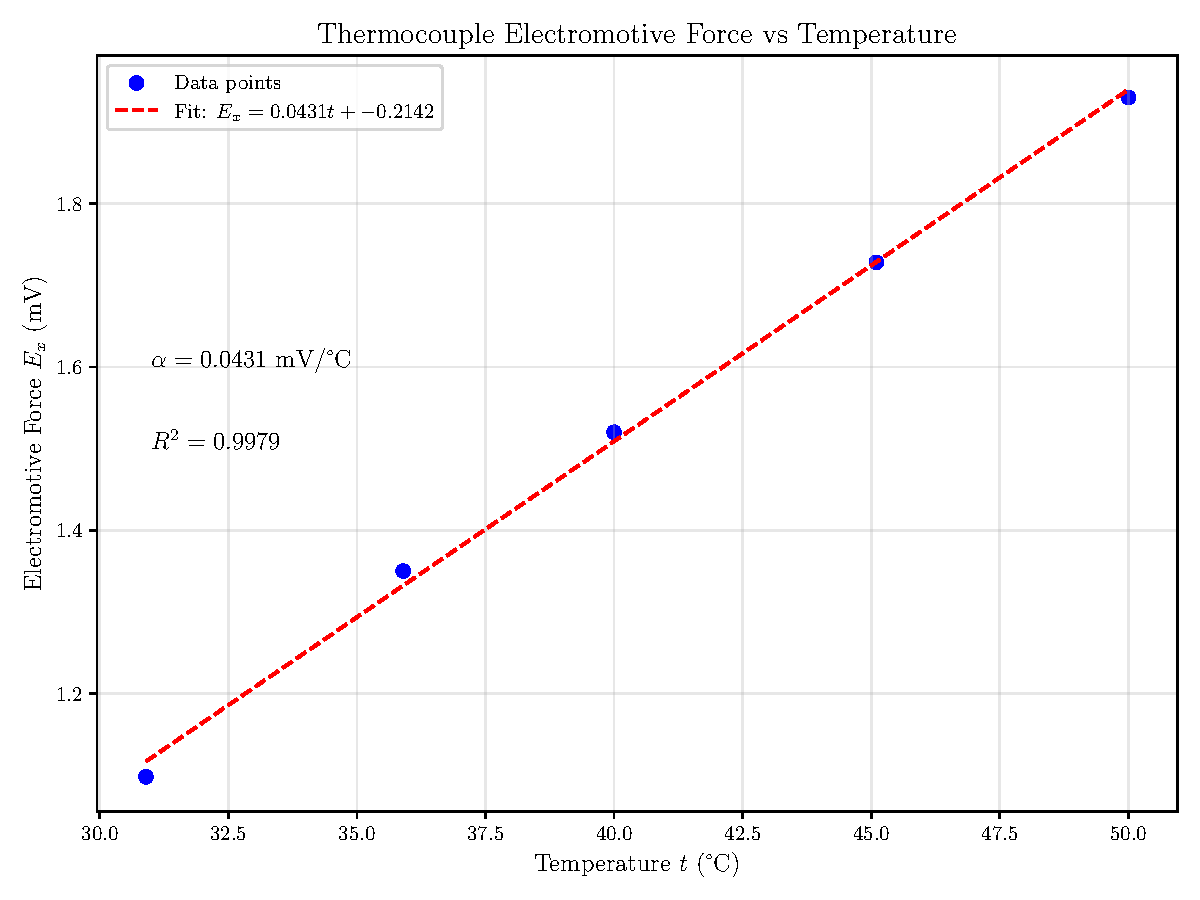
\includegraphics[width=0.6\textwidth]{./ex_vs_temp.pdf}
  \caption{温度-电动势曲线}
  \label{fig:温度-电动势曲线}
\end{figure}

\subsubsection{平衡电桥测铜电阻温度特性曲线}

\begin{table}[H]
	\centering
  \caption*{铜电阻：室温：$t=30.9^\circ C$  电阻：$R_x=58.8\Omega $ }
	\begin{tabular}{|c|c|c|c|c|c|}\hline
		温度$t^\circ C$   & 30.9 & 35.2 & 40.0 & 45.1 & 50.2 \\\hline
		电阻$R_x(\Omega)$ & 58.8 & 59.8 & 60.8 & 62.0 & 63.0\\\hline
	\end{tabular}
	\caption{平衡电桥测铜电阻的温度特性曲线}
\end{table}

根据以上数据，绘制温度-电阻曲线，通过线性拟合求得温度系数。结果如下：

\begin{figure}[H]
  \centering
  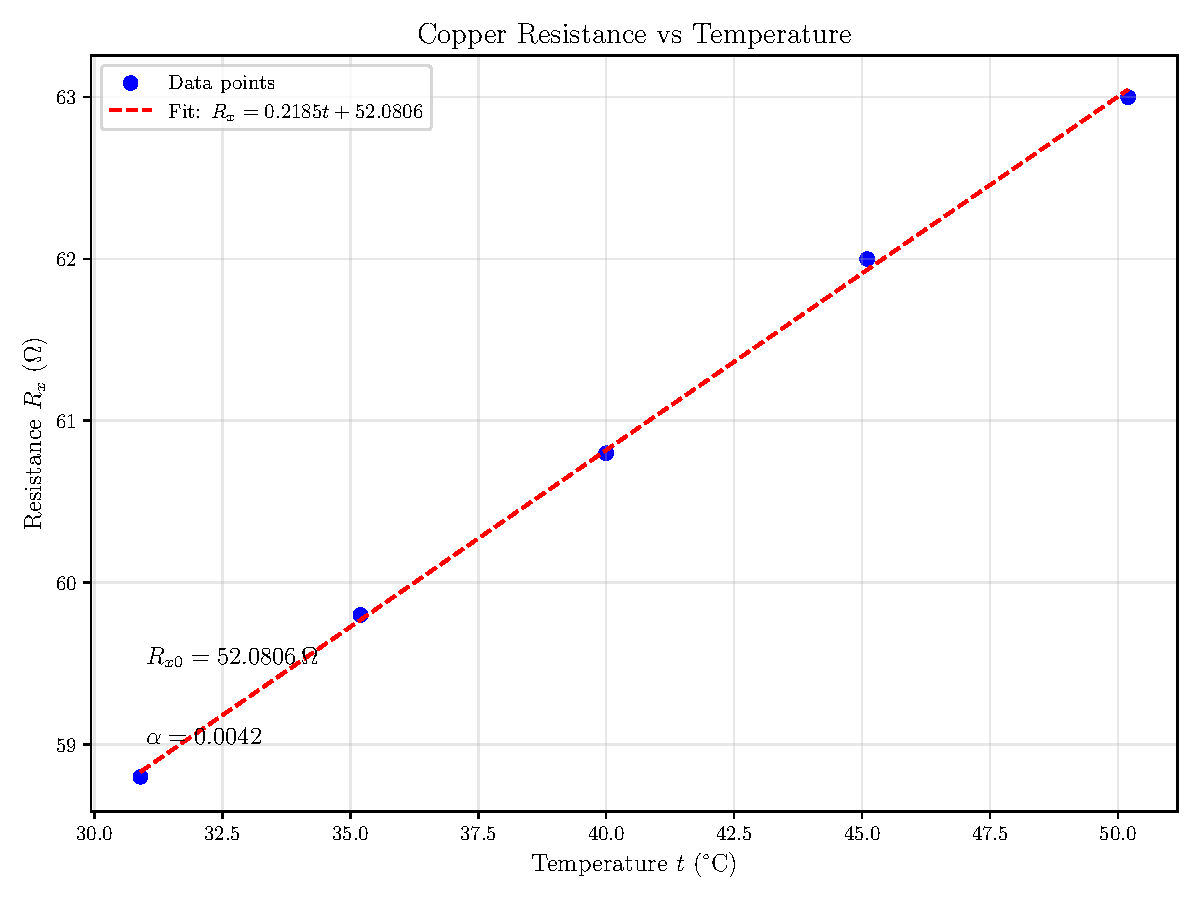
\includegraphics[width=0.6\textwidth]{./rx_vs_temp.pdf}
  \caption{温度-电阻曲线}
  \label{fig:温度-电阻曲线}
\end{figure}

根据回归直线数据可得直线的斜率 k = 0.2185，图像的相关指数 $R^2=0.9992$，表明直线拟合效果极佳，直线
的截距为 $R_0 = 52.0806\Omega$，根据公式测得铜的温度系数 $\alpha = 4.2 × 10^{-3}K^{-1}$，查询资料的铜电阻的温度系数为
  $0.0043K^{-1}$，测量值与实际值符合程度较高

\subsubsection{平衡电桥测热敏电阻温度特性曲线}

	\begin{table}[H]
		\centering
    \caption*{室温：$t=30.9^\circ C$电阻：$R_T=1944.0\Omega$\\}
		\begin{tabular}{|c|c|c|c|c|c|}\hline
			温度$t^\circ C$   & 30.9   & 35.4   & 40.0   & 45.1   & 50.4  \\\hline
			电阻$R_T(\Omega)$ & 1944.0 & 1601.0 & 1335.0 & 1091.0 & 890.0\\\hline
		\end{tabular}
		\caption{平衡电桥测热敏电阻温度特性曲线}
	\end{table}

根据以上数据，绘制温度的倒数与电阻的对数的曲线，通过线性拟合求得电阻的特性常数。结果如下：

\begin{figure}[H]
  \centering
  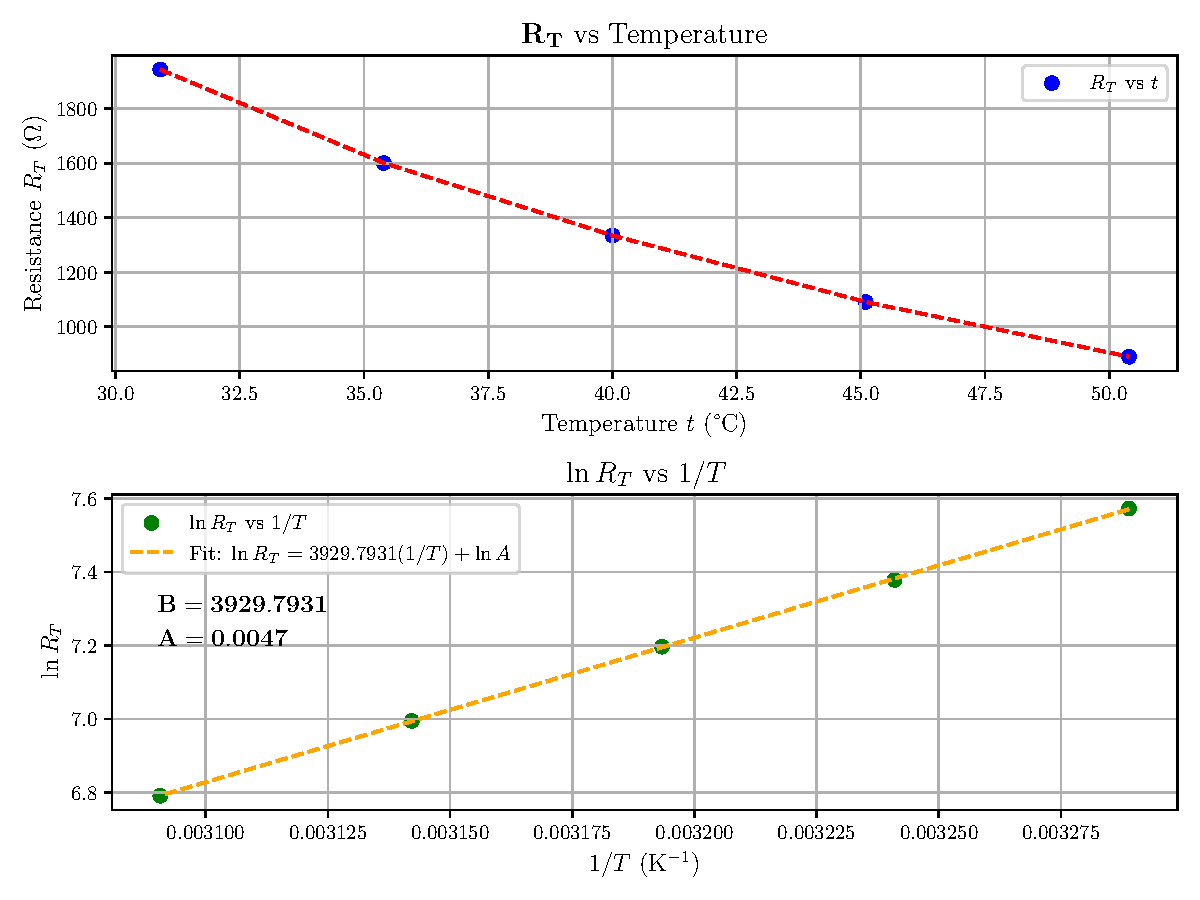
\includegraphics[width=0.6\textwidth]{./rt_vs_temp.pdf}
  \caption{热敏电阻温度曲线}
  \label{fig:热敏电阻温度曲线}
\end{figure}

\subsubsection{非平衡电桥测热敏电阻温度计}

\begin{table}[H]
	  温度区间：$30^\circ C$——$50^\circ C$\\
		热敏电阻特性常数：$A=0.004748151 \ \ B=3929.79$\\
		表头参数选择：$\lambda=-0.4V，m=-0.01V/^\circ C$\\	
		工作电源电压：$E=1.02416，R_2=908.87\Omega,\frac{R_2}{R_3}$=0.03066\\
		实际值：$R_2=1086.9\Omega,R_1=30.6\Omega,R_3=1000\Omega$\\
		
\centering
		\begin{tabular}{|c|c|c|c|c|c|}\hline
			温度$t^\circ C$     & 39.9   & 42.5   & 45.0   & 47.5   & 50.0 \\\hline
			测试电压$U_\circ(mv)$ & -399 & -424 & -447 & -470 & -493 \\\hline
			测试温度($^\circ C$)  & 39.9   & 43.4   & 44.7   & 47.0   & 49.3\\\hline
		\end{tabular}
		\caption{非平衡电桥热敏电阻温度计的设计}
	\end{table}

根据以上的图标可以看出，实际测量值与设定值的温度差距较小，表明非平衡电桥测热敏电阻温度计的设计是成功的。

\subsection{总结与思考}

\subsubsection*{1. 为什么在低温实验中常用四线式伏安法测温度，而工业仪表中常用非平衡电桥测温度？}

在低温实验中，温度测量的精度要求非常高，因为温度的微小变化可能会对实验结果产生显著影响。四线式伏安法能够精确测量电阻，从而间接测量温度。这种方法通过使用两根导线来施加电流，另外两根导线来测量电压降，从而避免了导线电阻对测量结果的影响。具体来说：

\begin{itemize}
    \item \textbf{电流导线}：用于施加电流，其电阻不会影响电压测量。
    \item \textbf{电压导线}：用于测量电压降，避免了电流导线电阻的影响。
\end{itemize}

这种方法特别适用于高精度的电阻测量，如低温下的温度测量，因为温度传感器（如铂电阻温度计）的电阻变化非常小，需要高精度的测量方法。

在工业仪表中，非平衡电桥（如惠斯通电桥）是一种常用的温度测量方法。这种方法通过将温度传感器（如热敏电阻或铂电阻）作为电桥的一个臂，通过测量电桥的不平衡电压来间接测量温度。非平衡电桥的优点包括：

\begin{itemize}
    \item \textbf{结构简单}：电桥结构简单，易于实现。
    \item \textbf{成本较低}：相对于四线式伏安法，非平衡电桥的成本较低。
    \item \textbf{易于集成}：可以与现有的工业控制系统集成，便于自动化控制和数据采集。
    \item \textbf{操作简便}：非平衡电桥操作简便，可测量的温度范围大，电桥的设置使测温系统容易根据实际需要进行调节，在不需要特别高精度的情况下，整个仪器性价比更高。
\end{itemize}

\subsubsection*{2. 工业仪表中使用的三线式非平衡电桥测温度是怎么消除引线电阻的？}

三线式非平衡电桥是一种改进的电桥结构，用于消除引线电阻对测量结果的影响。具体方法如下：

\begin{enumerate}
    \item \textbf{三线式结构}：
    \begin{itemize}
        \item \textbf{两根电流导线}：用于施加电流，分别连接到温度传感器的两端。
        \item \textbf{一根电压导线}：用于测量电压降，连接到温度传感器的两端。    \end{itemize}
    
    \item \textbf{消除引线电阻的影响}：
    \begin{itemize}
        \item \textbf{电流导线}：两根电流导线分别连接到温度传感器的两端，用于施加电流。电流导线的电阻不会影响电压测量。
        \item \textbf{电压导线}：电压导线连接到温度传感器的两端，用于测量电压降。分析实验的中测量电路可发现，在搭建过程中可以要求电桥两臂上引线的电阻相等，这样这部分电阻实际上被抵消，外部电路的电阻对电桥本身不产生影响，从而引线的电阻被消除。
    \end{itemize}

\end{enumerate}

\subsubsection{实验心得}


1. 实验中加热装置的散热速度较慢，为了提高实验效率，可以在加热到指定温度后，依次测量热电偶、铜电阻和热敏电阻的阻值，再进行下一组数据的测量。然而，这种测量方法存在一个缺点，即控温仪的温度维持时间有限，因此后续的测量点可能会存在温度偏差。为了减少这个影响，最好在每次测量阻值时，记录下对应的温度。可以这样做的原因是，再以温度为横坐标作图时，不需要温度为严格的整数。同时，实验中加热装置加热速度很快，并且预置温度的准确性不够高，常常在前几秒超过预置温度，一段时间后又低于预置温度。因此，在进行实验时不应该以预置温度为准，而是应当时刻关注温控装置的读数。

2. 最终得到的热电偶温度特性曲线虽然是线性的，但它与原点并不重合，且在x轴上有负的截距。我们推测可能是因为热电偶的冷端被卡在冰块中，导致实际温度低于0°C。在数据处理时，考虑到实验是在课程时间内完成的，且设备没有拆除，我后来检查发现，实际上热电偶的冷端接触到了杯底。尽管调整热电偶的位置很难使其冷端完美悬浮在溶液中，但在类似实验中，改进实验装置并增加固定装置会有助于避免这种问题。

\end{document}

% VScode 常用快捷键：

% F2:                       变量重命名
% Ctrl + Enter:             行中换行
% Alt + up/down:            上下移行
% 鼠标中键 + 移动:           快速多光标
% Shift + Alt + up/down:    上下复制
% Ctrl + left/right:        左右跳单词
% Ctrl + Backspace/Delete:  左右删单词    
% Shift + Delete:           删除此行
% Ctrl + J:                 打开 VScode 下栏(输出栏)
% Ctrl + B:                 打开 VScode 左栏(目录栏)
% Ctrl + `:                 打开 VScode 终端栏
% Ctrl + 0:                 定位文件
% Ctrl + Tab:               切换已打开的文件(切标签)
% Ctrl + Shift + P:         打开全局命令(设置)

% Latex 常用快捷键：

% Ctrl + Alt + J:           由代码定位到PDF


